% Liveness-guidance workflow figure, shared across LRU-Live, SRRIP-Live, and
% IPV-Live. Style modeled on Mazumdar et al. (HPCA 2021) Fig. 6 / Fig. 8: split
% into (a) lookup, (b) fill, and (c) eviction sub-flowcharts. Set dueling is
% intentionally omitted here for clarity; the three policies share this exact
% shape and differ only in the concrete action taken at each policy-specific
% step, listed in Table~\ref{tab:mechanism_actions}.
% Wrapped in \resizebox so it always fits its minipage column.
\usetikzlibrary{shapes.geometric, arrows.meta, positioning, fit, calc}

\tikzset{
  wfstart/.style   = {rectangle, rounded corners, draw=black, thick, fill=gray!15,
                       minimum width=2.6cm, minimum height=0.55cm, text width=2.4cm,
                       align=center, font=\scriptsize, inner sep=2pt},
  wfproc/.style    = {rectangle, draw=black, fill=blue!8,
                       minimum width=2.6cm, minimum height=0.6cm, text width=2.4cm,
                       align=center, font=\scriptsize, inner sep=2pt},
  wfdoa/.style     = {rectangle, draw=black, fill=red!10,
                       minimum width=2.4cm, minimum height=0.6cm, text width=2.2cm,
                       align=center, font=\scriptsize, inner sep=2pt},
  wfbypass/.style  = {rectangle, draw=black, thick, fill=red!35,
                       minimum width=2.4cm, minimum height=0.6cm, text width=2.2cm,
                       align=center, font=\scriptsize, inner sep=2pt},
  wfalive/.style   = {rectangle, draw=black, fill=green!10,
                       minimum width=2.4cm, minimum height=0.6cm, text width=2.2cm,
                       align=center, font=\scriptsize, inner sep=2pt},
  wfdecision/.style = {diamond, draw=black, fill=orange!12, aspect=2.2,
                       text width=2.6cm, align=center, font=\scriptsize, inner sep=1pt},
  wfarrow/.style   = {thick, -{Latex[length=1.8mm]}},
  wflabel/.style   = {font=\tiny, fill=white, inner sep=1pt}
}

% ============================================================================
% Figure: shared liveness-guidance workflow
% ============================================================================
\begin{figure*}[t]
\centering
% --- (a) Hit --------------------------------------------------------------
\begin{minipage}[t]{0.32\textwidth}
\centering
\resizebox{\linewidth}{!}{%
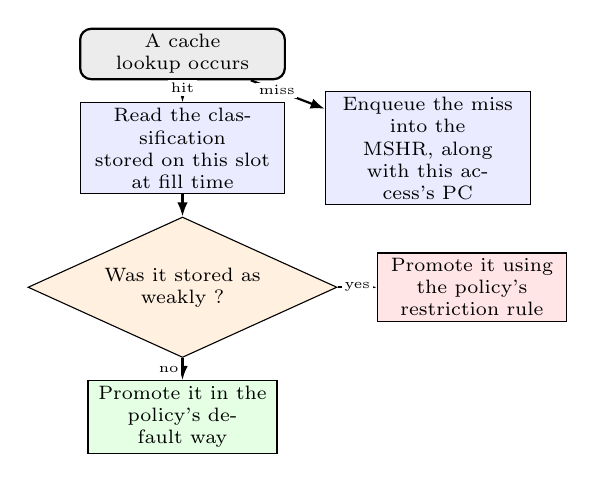
\begin{tikzpicture}[node distance=0.28cm and 0.5cm]
  \node (start) [wfstart] {A cache lookup occurs};
  \node (readcls) [wfproc, below=of start] {Read the classification\\stored on this slot\\at fill time};
  \node (missbox) [wfproc, right=of readcls] {Enqueue the miss\\into the MSHR, along\\with this access's PC};
  \node (clsdec) [wfdecision, below=of readcls] {Was it stored as\\weakly \doa?};
  \node (doahit) [wfdoa, right=of clsdec] {Promote it using\\the policy's\\restriction rule};
  \node (alivehit) [wfalive, below=of clsdec] {Promote it in the\\policy's default way};

  \draw [wfarrow] (start) -- node[wflabel,pos=0.35] {hit} (readcls);
  \draw [wfarrow] (start) -- node[wflabel,pos=0.35] {miss} (missbox);
  \draw [wfarrow] (readcls) -- (clsdec);
  \draw [wfarrow] (clsdec) -- node[wflabel] {yes} (doahit);
  \draw [wfarrow] (clsdec) -- node[wflabel,left] {no} (alivehit);
\end{tikzpicture}}
\footnotesize (a) Lookup
\end{minipage}
\hfill
% --- (b) Fill --------------------------------------------------------------
\begin{minipage}[t]{0.32\textwidth}
\centering
\resizebox{\linewidth}{!}{%
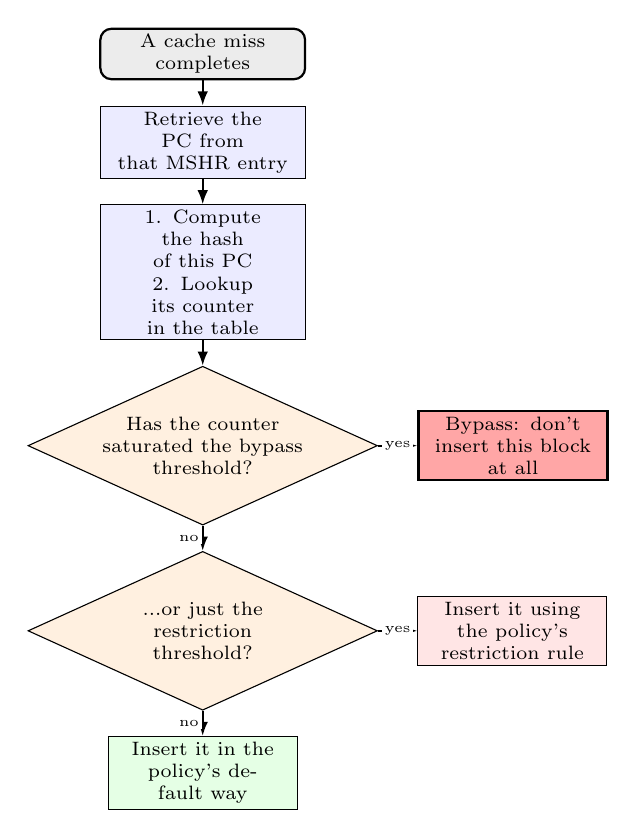
\begin{tikzpicture}[node distance=0.32cm and 0.5cm]
  \node (start) [wfstart] {A cache miss completes};
  \node (retrieve) [wfproc, below=of start] {Retrieve the PC from\\that MSHR entry};
  \node (lookup) [wfproc, below=of retrieve] {1. Compute the hash\\of this PC\\2. Lookup its counter\\in the table};
  \node (strongdec) [wfdecision, below=of lookup] {Has the counter\\saturated the bypass\\threshold?};
  \node (bypass) [wfbypass, right=of strongdec] {Bypass: don't\\insert this block\\at all};
  \node (weakdec) [wfdecision, below=of strongdec] {...or just the\\restriction\\threshold?};
  \node (doains) [wfdoa, right=of weakdec] {Insert it using\\the policy's\\restriction rule};
  \node (aliveins) [wfalive, below=of weakdec] {Insert it in the\\policy's default way};

  \draw [wfarrow] (start) -- (retrieve);
  \draw [wfarrow] (retrieve) -- (lookup);
  \draw [wfarrow] (lookup) -- (strongdec);
  \draw [wfarrow] (strongdec) -- node[wflabel] {yes} (bypass);
  \draw [wfarrow] (strongdec) -- node[wflabel,left] {no} (weakdec);
  \draw [wfarrow] (weakdec) -- node[wflabel] {yes} (doains);
  \draw [wfarrow] (weakdec) -- node[wflabel,left] {no} (aliveins);
\end{tikzpicture}}
\footnotesize (b) Fill
\end{minipage}
\hfill
% --- (c) Eviction ------------------------------------------------------------
\begin{minipage}[t]{0.32\textwidth}
\centering
\resizebox{\linewidth}{!}{%
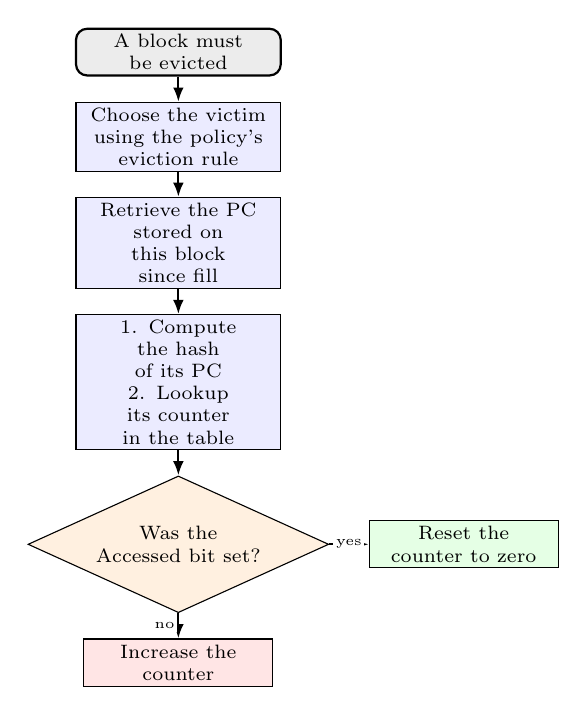
\begin{tikzpicture}[node distance=0.32cm and 0.5cm]
  \node (start) [wfstart] {A block must be evicted};
  \node (pick) [wfproc, below=of start] {Choose the victim\\using the policy's\\eviction rule};
  \node (retrieve) [wfproc, below=of pick] {Retrieve the PC\\stored on this block\\since fill};
  \node (lookup) [wfproc, below=of retrieve] {1. Compute the hash\\of its PC\\2. Lookup its counter\\in the table};
  \node (acc) [wfdecision, below=of lookup] {Was the\\Accessed bit set?};
  \node (reset) [wfalive, right=of acc] {Reset the\\counter to zero};
  \node (inc) [wfdoa, below=of acc] {Increase the\\\doa counter};

  \draw [wfarrow] (start) -- (pick);
  \draw [wfarrow] (pick) -- (retrieve);
  \draw [wfarrow] (retrieve) -- (lookup);
  \draw [wfarrow] (lookup) -- (acc);
  \draw [wfarrow] (acc) -- node[wflabel] {yes} (reset);
  \draw [wfarrow] (acc) -- node[wflabel,left] {no} (inc);
\end{tikzpicture}}
\footnotesize (c) Eviction
\end{minipage}
\caption{Shared operation of liveness guidance across \lru-Live, \srrip-Live, and \ipv-Live. Each PC has a per-PC \doa counter, checked against two thresholds: saturating the restriction threshold still inserts the block, but with reduced protection, while saturating the higher bypass threshold skips insertion entirely. An eviction updates the counter based on whether the Accessed bit was set. The three policies share this exact flow and differ only in their concrete insertion and promotion rules.}
\label{fig:liveness_workflow}
\end{figure*}

% ============================================================================
% Table: concrete per-policy actions
% ============================================================================
\begin{table}[t]
\centering
\caption{Concrete action per policy for each step of Figure~\ref{fig:liveness_workflow}. $N = \text{NUM\_WAY}$; maxRRPV $=3$. Values shown are each policy's default (non-dueling) configuration.}
\label{tab:mechanism_actions}
\footnotesize
\begin{tabular}{@{}l l l l@{}}
\toprule
Step & \lru-Live & \srrip-Live & \ipv-Live \\
\midrule
\doa insert   & $N{-}1{-}\lfloor 2N/3\rfloor$ & $2$ & $\text{ipv}_{\doa}[N]$ \\
Alive insert  & $N{-}1$          & $2$ & $\text{ipv}_{\text{alive}}[N]$ \\
\doa hit      & $N{-}1$ (or capped$^{*}$) & $\to 2$ (partial) & $\text{ipv}_{\doa}[\text{rank}]$ \\
Alive hit     & $N{-}1$          & $\to 0$ (full) & $\text{ipv}_{\text{alive}}[\text{rank}]$ \\
Victim pick   & lowest rank      & first @ maxRRPV & tail \\
\bottomrule
\end{tabular}

\vspace{2pt}
\raggedright\footnotesize *With \texttt{LRU\_LIVE\_HIT\_INIT=1}, a \doa hit promotes only to the class's initial insertion position rather than to MRU; default is full MRU promotion for all hits.
\end{table}
